%!TEX root = ./main.tex
\section*{Important Hypothesis (Daniel-Saúl)}
    \paragraph{Permanent immunity}
    Accordingly to \cite{WHO}, Dengue infection caused by a DEN-i serotype induces long-life immunity to reinfection for this strain. Also,  a recovered individual previously infected with DEN-i Dengue serotype, acquires partial immunity to a different serotype for about a period of two years \cite{Reich2013}. As our study focuses on a single year dynamics, we assume that a susceptible individual who has never get infected before, could obtain Dengue by any of serotypes DENV-1, or DENV-2, and then becoming recovered to any strain for the rest of the year. 
    
    %
    \paragraph{ADE hypothesis}
    The processes and factors that produce \ac{DHF} are still unclear. Different factors have
    been observed to be responsible for DHF \cite{Martina2009}. However, one of the most predominant hypothesis claims that reinfection with a different serotype enhances the probability of developing plasma vascular permeability---the \ac{ADE} hypothesis \citep[see, e.g.][p. 295]{Halstead1992}, \cite{Guzman2013}. We consider in our formulation the ADE hypothesis, that 
    is, only a fraction of the second reinfection with serotype \ac{DENV-2} develops vascular leaking. Additionally, a second consequence of the ADE hyphotesis, is that the susceptibility of acquiring dengue a second time, is increased \cite{Recker2009}. \\
    %But there also exist studies that report first infection DHF cases \cite{Debast1993}.
%
    \paragraph{\ac{DENV-2} report circulation in Hermosillo}



    We assume that the $X\%$ (pending) of the \ac{DCF} are asymptomatic, whereas for 
    \ac{DHF}  all the cases are reported. 
    
    
    Therefore, the class $Y_{-1}^{[h]}$ accounts for
    all the \ac{DHF} cases, whereas a fraction $p=0.05$ of the sum 
    $I_1+ I_2 + Y_{-1}^{[c]}$ represent the confirmed cases of \ac{DCF}. (75\% is the amount of asymptomatic according to literature)

    \tinytodo{Incluir citas de los 
        porcentages de asintomáticos,
        http://www.who.int/%
        en/news-room/fact-sheets/%
        detail/dengue-and-severe-dengue %
        says that about% 
        75$\%$ is asymptomatic}

    \todo{chastel2012.pdf}
    \paragraph{Homogeneity about the early outbreak stage}

    Define the infection forces as
    \begin{equation}
        \begin{aligned}
            A_{I_1} &=
                \frac{\beta_Mb}{N_H} I_1, \qquad
            A_{I_2}=
                \frac{\beta_Mb}{N_H} I_2,
        \\
            A_{Y_{-1}^{[h]}}&=
            \frac{\beta_Mb}{N_H} Y_{-1} ^{[h]}, \qquad
            A_{Y_{-1}^{[c]}}=
                \frac{\beta_Mb}{N_H} Y_{-1}^{[c]},
        \\
            B_{M_1} &= 
                \frac{\beta_Hb}{N_H}M_1, \qquad
            B_{M_2}=
                \frac{\beta_Hb}{N_H}M_2 ~.
        \end{aligned}
    \end{equation}
    \paragraph{Vector transmission dynamics}
    Define
    $$
        A_{\bullet}:=
            A_{I_1} + A_{I_2} + A_{Y_{-1}^{[h]}} + 
            A_{Y_{-1}^{[c]}}
    $$
    as the total human infection force, that is, 
    the sum of all
    human contributions to the vector infection. 
    Then we describe the mosquito disease dynamics 
    by 
    \begin{equation}
        \begin{aligned}
            \\
            \frac{dM_S}{dt}&=
                \Lambda_M
                - A_{\bullet} M_S
                - \mu_M M_S
            \\
            \frac{dM_1}{dt}&=
                A_{I_1}  M_S - \mu_M M_1
            \\
            \frac{dM_2}{dt} &=
                \left(
                    A_{I_2}+A_{Y_{-1}^{[h]}}+A_{Y_{-1}^{[c]}}
                \right) 
                M_S-\mu_M M_2
        \end{aligned}
    \end{equation}
    Here $M_S$, is the vector susceptible class and
    $M_1$, $M_2$ respectively denotes the vector 
    Infected classes with \ac{DENV-1}
    and \ac{DENV-2}.
    \paragraph{Host disease dynamics}
        Susceptible individuals ($S$) become infected for the first time
        with DENV-1 or DENV-2 after  a successful mosquito bite and move
        to classes $I_1$ and $I_2$, respectively. From here, they remain
        in the infected class for $1/\alpha_c$ time units, after which,
        move to a recovered class $R_S$.  As we are interested in a one
        year dynamics, for the rest of the epidemic they become immune to
        any serotype. A second class of susceptible individuals $S_{-1}$,
        consist on those who acquired DENV-1 in previous years and in the
        current year are susceptible only to DENV-2. Such individuals
        become infected with DENV-2 when exposed to infected mosquitoes
        with that serotype. In \cite{OhAinle2011} and
        \cite{Sangkawibha1984} it was observed that a more severe version
        of dengue occurs (might occur?) when an individual acquires dengue
        for a second time, and this happens to be DENV-2. Based on this
        assumption, an individual from $S_{-1}$ moves to $Y_{-1}^{[c]}$ or
        $Y_{-1}^{[h]}$, if the infection leads to DF or DHF, respectively.
        Finally, these infected individuals move to the recovered class
        $R_{S_{-1}}$ at rates $\alpha_c$ and $\alpha_h$, respectively. For
        our model, $\mu_H$ is the human death rate; $b$ is the number of
        bites per week per mosquito and $\beta_H$ is the effectiveness of
        the bite. From the current hypothesis our model is given by    

%Assuming sufficient density of vectors, we 
%describe the \ac{DCF} and \ac{DHF},
%using a cross infection mechanism similar to the 
%reported in \cite{Feng1997a}. 
%Our version allows a hemorrhagic description of 
%the Infected human population 
%with serotype $i$---see 
%\Cref{tbl:variable_description,tbl:parameter_description}
%to variable and parameter description. The symbol 
%$I_{i}$ represents the human infected 
%pupulation with serotype $i$,
%which never was infected before, while 
%$Y_{-i}^{[\star]}$ denotes the 
%number of humans which are immune to serotype 
%$i$ at the time of the 
%present outbreak and develops dengue of type 
%$\star$ (DCF or DHF).
%Then $S_{-i}$ are the individuals who were 
%infected with serotype $i$ in the 
%previous outbreak, and at the current time, are 
%susceptible only to a serotype different of $i$.
%Dengue cross infection.

\begin{equation}\label{eqn:model_two_strains1}
    \begin{aligned}
        \frac{dS}{dt} &=
            \mu_HN_S - (B_{M_1} + B_{M_2}) S
            -\mu_H S
        \\
        \frac{dI_1}{dt} &=
            B_{M_1} S
            -(\alpha_c + \mu_H) I_1
        \\
        \frac{dI_2}{dt} &=
            B_{M_2} S
            -(\alpha_c + \mu_H)I_2
        \\
        \frac{dR_S}{dt}&=\alpha_c I_2-\mu_H R_S
        \\
        \frac{dS_{-1}}{dt} &=
            \mu_HN_{S_{-1}}- \sigma B_{M_2} S_{-1}-\mu_H S_{-1}
        \\
        \frac{dY_{-1} ^{[c]} }{dt} &=
            (1 - \theta) \sigma B_{M_2} S_{-1}
            -(\alpha_c + \mu_H) Y_{-1} ^ {[c]}
        \\
        \frac{dY_{-1}^{[h]}}{dt} &=
            \theta \sigma B_{M_2} S_{-1}
            -(\alpha_h + \mu_H)Y_{-1} ^{[h]} 
        \\
        \frac{dR_{S_{-1}}}{dt} &= 
            \alpha_c Y_{-1} ^{[c]}
            + \alpha_h Y_{-1} ^ {[h]} - \mu_H R
    \end{aligned}
\end{equation}
    Here, we take $N_H=N_S+N_{S_{-1}}$ as the total number of individuals.
    For our formulation $N_H, N_S$ and $N_{S_{-1}}$ remain constant. $N_S$
    is the total number of individuals that are involved in the first
    infection dynamics ($N_S = S +I_1+I_2+R_S$). On the other hand
    $N_{S_{-1}}$ is the total number of individuals involved in the
    reinfection dynamics ($N_{S_{-1}}=S_{-1}+Y_1^{[c]}+
    Y_1^{[h]}+R_{S_1}$). Also, the recovered individuals in both classes
    can be considered as a single recovered class $R=R_S+R_{S_{-1}}$ as
    our dynamics are taken only for one year. Then, our equations become

\begin{equation}\label{eqn:model_two_strains2}
    \begin{aligned}
        \frac{dS}{dt} &=
            \mu_HN_S - (B_{M_1} + B_{M_2}) S
            -\mu_H S
        \\
        \frac{dI_1}{dt} &=
            B_{M_1} S
            -(\alpha_c + \mu_H) I_1
        \\
        \frac{dI_2}{dt} &=
            B_{M_2} S
            -(\alpha_c + \mu_H)I_2
        \\
        \frac{dS_{-1}}{dt} &=
            \mu_HN_{S_{-1}}- \sigma B_{M_2} S_{-1}-\mu_H S_{-1}
        \\
        \frac{dY_{-1} ^{[c]} }{dt} &=
            (1 - \theta) \sigma B_{M_2} S_{-1}
            -(\alpha_c + \mu_H) Y_{-1} ^ {[c]}
        \\
        \frac{dY_{-1}^{[h]}}{dt} &=
            \theta \sigma B_{M_2} S_{-1}
            -(\alpha_h + \mu_H)Y_{-1} ^{[h]} 
        \\
        \frac{dR}{dt} &= 
            \alpha_c 
                \left(
                    I_1 + I_2 + Y_{-1} ^{[c]}
                \right)
            + \alpha_h Y_{-1} ^ {[h]} - \mu_H R
    \end{aligned}
\end{equation}


\todo{Fix $\Lambda _{\cdot} = N$. }
\todo{Include information about the 2 strains}
\begin{figure}[htb]
	\centering
	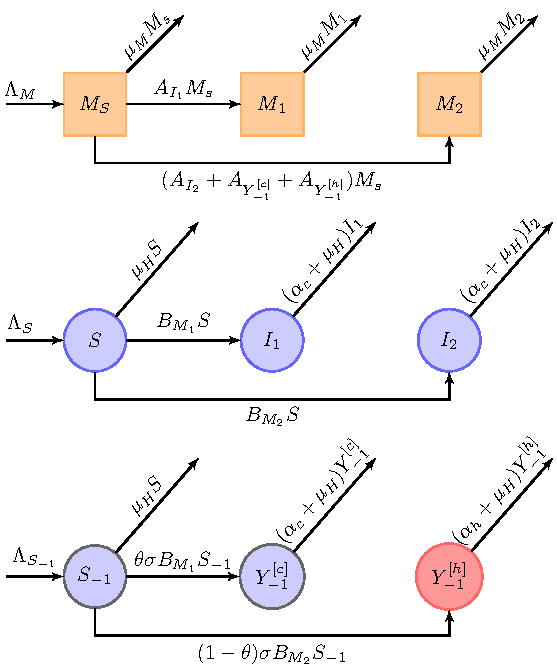
\includegraphics[width=\linewidth]{disiase_flow.pdf}
	\caption{Flow diagram of model \eqref{eqn:model_two_strains}}.
	\label{fig:disiaseflow}
\end{figure}
%
\begin{table*}[h!]
	\begin{center}
		\begin{tabular}{rl}
			\toprule
			Symbol		&	\multicolumn{1}{c}{Meaning}
			\\
			\midrule
			$M_S$
				& Number of susceptible mosquitoes.
			\\
			$M_1$, $M_2$
				&
				 Number of infected mosquitoes with virus
				\\
				& 
				serotype \ac{DENV-1} or \ac{DENV-2}.
			\\
			$S$
				&
				Susceptible host population which, 
				\\
				& never has acquired dengue.
			\\
			$S_{-1}$
			&
				Susceptible host population 
				which is immune to
			\\
			&
				serotype $1$.
			\\
			$I_1$, $I_2$
			&
				First time infected host population by 
			\\
				& serotype $1$ and $2$, respectively.
			\\
				$Y_{-1}^{[h]}$,
				$Y_{-1}^{[c]}$
				&
				Second time infected host population with 
				\\
				&
				serotype 2, with \ac{DHF} and \ac{DCF}, 
                \\
                &
                respectively.
			\\
		\bottomrule
		\end{tabular}
	\end{center}
	\caption{
		Meaning of variables. 
		Here we omit the explicit dependence of
		time.
	}\label{tbl:variable_description}
\end{table*}

%
%
\paragraph{Basic reproductive number}
    The disease free equilibrium results
$$
    FDE=
    \left(
        \frac{\Lambda_M}{\mu_M},
        0,
        0,
        N_H - N_{S_{-1}},
        0,
        N_{S_{-1}},
        0,
        0,
        0
    \right).
$$
\todo{get a relation for the initial grow phase parameter}
Using the next generation operator method 
reported as in \cite{Feng1997a}, we obtain
the basic reproductive number
%\begin{equation}
%   \begin{aligned}
%       \pi_R & :=
%           \frac{\beta_H \beta_M b^2 \Lambda_M}{
%               \mu_M ^ 2  N_H ^ 2 
%       }
%   \\
%       R_{01} & := 
%           \pi_R
%           \left(
%               \frac{N_H - N_{S_{-1}}}{ \alpha_c + \mu_H}
%               +
%               \frac{(1- \theta ) \sigma N_{S_{-1}}}{ \alpha_c + \mu_H}
%           \right)
%       \\
%       R_{02}& :=
%           \pi_R
%               \frac{
%                   \sigma \theta N_{S_{-1}}
%               }{\alpha_h + \mu_H},
%\qquad
%   \\
%   \mathcal{R}_0 & :=
%           \sqrt{ R_{01}+R_{02} }.
%   \end{aligned}
%\end{equation}
%
\begin{equation}
    \begin{aligned}
        \psi &:= \frac{\beta_MbN_M}{\mu_MN_H}
        \\
        R_{0c} & := \sqrt{
            \psi
            \left(
                \frac{\beta_HbN_S}{ (\alpha_c + \mu_H)N_H}
                +
                \frac{\beta_Hb(1- \theta ) \sigma N_{S_{-1}}}{ (\alpha_c + \mu_H)N_H}
            \right)}
        \\
        R_{0h}& :=\sqrt{
            \left(\frac{\beta_MbN_M}{\mu_MN_H}\right)
                \left(\frac{
                    \sigma \theta N_{S_{-1}}
                }{(\alpha_h + \mu_H)N_H}\right)}
%       \qquad
    \\
    \mathcal{R}_0 & :=
            \sqrt{ R_{0c}^2+R_{0h}^2 }.
    \end{aligned}
\end{equation}

        In this equation, $R_{0c}$ and $R_{0h}$, are the basic reproductive numbers 
    for classical and hemorrhagic dengue cases, respectively. From here, $R_0$ 
    provides a measure of how DF and DHF infected people influence the presence of 
    new dengue cases (Either DF or DHF). $R_{0h}$ measures the new hemorrhagic 
    cases that arise from one hemorrhagic infected individual in a population of 
    $N_{S_{-1}}$ susceptible to strain 2 individuals, meanwhile $R_{oc}$ provides a 
    measure of how many new individuals will obtain DC fever (DF?) from an individual 
    that has or has not have acquired dengue previously (from an individual that has either
    DF or DHF).

        Observe that this $R_0$ differs in some way to the traditional $R_0$ where two
    different serotypes are involved (\cite{Feng1997a} include citations of $R_0$ 
    for two serotypes).
    This follows from the idea that we are interested in classic and hemorrhagic
    cases rather than the predominance of a serotype.




